
\documentclass[11pt]{article}
%\usepackage[top=20mm,left=20mm,right=20mm,bottom=15mm,a4paper]{geometry} % see geometry.pdf on how to lay out the page. There's lots.
\usepackage[top=20mm,left=20mm,right=20mm,bottom=15mm,headsep=15pt,footskip=15pt,a4paper]{geometry} % see geometry.pdf on how to lay out the page. There's lots.
%\geometry{a4paper} % or letter or a5paper or ... etc
% \geometry{landscape} % rotated page geometry
\usepackage[round]{natbib}
\setlength{\bibsep}{0.0pt}
\usepackage{color}
\usepackage{times}
%\usepackage[T1]{fontenc}
%\usepackage{mathptmx}
\usepackage{tikz-dependency}
\usepackage{enumitem}
%\usepackage{times}

\usepackage[procnames]{listings}
\usepackage{color}
 
 

% See the ``Article customise'' template for come common customisations
\newcommand{\refeq}[1]{Equation~\ref{eq:#1}}
\newcommand{\reffig}[1]{Figure~\ref{fig:#1}}
\newcommand{\reftab}[1]{Table~\ref{tab:#1}}
\newcommand{\refsec}[1]{\textsection\ref{sec:#1}}
\newcommand{\newsec}[2]{\section{#1}\label{sec:#2}\noindent}
\newcommand{\newsubsec}[2]{\subsection{#1}\label{sec:#2}\noindent}
\newcommand{\argmax}{\operatornamewithlimits{argmax}} 
\newcommand{\argmin}{\operatornamewithlimits{argmin}} 

\makeatletter         
\def\@maketitle{   % custom maketitle 
\begin{center}%
{\bfseries \@title}%
{\bfseries \@author}%
\end{center}%
\smallskip \hrule \bigskip }

% custom section 
\renewcommand{\section}{\@startsection
{section}%                   % the name
{1}%                         % the level
{0mm}%                       % the indent
{-0.8\baselineskip}%            % the before skip
{0.3\baselineskip}%          % the after skip
{\bfseries\large}}% the style

% custom subsection 
\renewcommand{\subsection}{\@startsection
{subsection}%                   % the name
{2}%                         % the level
{0mm}%                       % the indent
{-0.8\baselineskip}%            % the before skip
{0.3\baselineskip}%          % the after skip
{\bfseries\large}}% the style

\renewcommand{\paragraph}{%
  \@startsection{paragraph}{4}%
  {\z@}{1.5ex \@plus 1ex \@minus .2ex}{-1em}%
  {\normalfont\normalsize\bfseries}%
}\makeatother

%\title{{\LARGE Universal Parser (UP)}\\[-8mm]
%\includegraphics[height=8mm]{RUPA}~~~~~~~~~~~~~~~~~~~~~~~~~~~~~~~~~~~~~~~~~~~~~~~~~~~~~~~~~~~~~~~~~~~~~~~~~~~\includegraphics[height=8mm]{RUPA}}
\title{{\LARGE Natural Language Processing}\\[1.5mm]{\large Assignment 6: Hidden Markov Models}}
\author{}
\date{} % delete this line to display the current date

%%% BEGIN DOCUMENT
\begin{document}

\definecolor{keywords}{RGB}{255,0,90}
\definecolor{comments}{RGB}{0,0,113}
\definecolor{red}{RGB}{160,0,0}
\definecolor{green}{RGB}{0,150,0}
 
\lstset{language=Python, 
        basicstyle=\ttfamily\small, 
        keywordstyle=\color{keywords},
        commentstyle=\color{comments},
        stringstyle=\color{red},
        showstringspaces=false,
        identifierstyle=\color{green},
        procnamekeys={def,class}}

\maketitle
%\tableofcontents
%\vspace{3mm}
\vspace{-2mm}
\newsec{Introduction}{intro}%
In this assignment, we are going to explore the use of Hidden Markov Models for predictive text entry, as used for text messaging on pre-smartphone mobile phones.
This is an exercise in mathematical modeling and reasoning, so you will not be asked to do any programming or empirical evaluation this time.

\newsec{The problem}{problem}%
Assume we have a keypad that looks like this:
\begin{center}
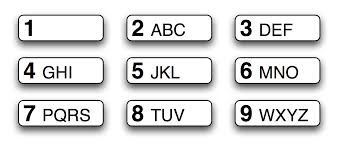
\includegraphics[scale=0.5]{pics/keypad.jpeg}
\end{center}
When used to produce text messages on a mobile phone, this device produces a sequence of numbers that can represent multiple sequences of characters. 
For example, to type the word {\em box}, you would produce the key sequence 269. But the same sequence would be produced also for the word {\em bow}. 
The predictive text entry problem can be seen as the problem of predicting the most probable word given a sequence of numbers (keys).
\newsec{Build a model}{model}%
The predictive text entry problem can be seen as a sequence tagging problem, where we are given observable sequence of numbers and are required to
find hidden sequences of characters. It is therefore a good fit for a Hidden Markov Model. Your first task is to define the model structure.
\begin{itemize}[noitemsep,topsep=0.2cm]
\item What are the (hidden) states of the model?
\item What are the output symbols of the model?
\end{itemize}

\newsec{Estimate probabilities}{estimate}%
Once you have defined the model structure (states and symbols), there are two probability distributions that need to be estimated.
\begin{itemize}[noitemsep,topsep=0.2cm]
\item How would you estimate the emission probabilities $P(\mbox{symbol}|\mbox{state})$?
\item How would you estimate the transition probabilities $P(\mbox{new state}|\mbox{previous state})$?
\end{itemize}

\newsec{Use model for decoding}{decode}%
Given estimates of the probability distribution, the model can be used to decode key sequences by finding the most probable word.
\begin{itemize}[noitemsep,topsep=0.2cm]
\item How would you compute the probability that 269 corresponds to {\em box} in your model?
\item How would you compute the most probable word corresponding to 269 in your model?
\end{itemize}
\textbf{Note:} You are not supposed to carry out any concrete computations here, only show as a matter of principle how to do the computations.

\newsec{Submit the assignment}{submit}%
Submit the following to {\tt nlp-course@stp.lingfil.uu.se}: 
\begin{itemize}[noitemsep,topsep=0.2cm]
\item Well motivated answers to all questions in Section~\ref{sec:model}--\ref{sec:decode}.
\end{itemize}

\end{document}